%%%%%%%%%%%%%%%%%%%%%%%%%%%%%%%%%%%%%%%%%%%%%%%%%%%%%%%%%%%%%%%%%%%%%%%%%%%%%%%%%%%%%%%%%%%%%%%%%%%
% Synthetic PIV:
%%%%%%%%%%%%%%%%%%%%%%%%%%%%%%%%%%%%%%%%%%%%%%%%%%%%%%%%%%%%%%%%%%%%%%%%%%%%%%%%%%%%%%%%%%%%%%%%%%%
\chapter{Module 2: Synthetic Image Generation}\label{ch:sypiv}
The uncertainty of the imaging phase and its interrogation phase in PIV contributes significantly to the total generated uncertainty. This has been demonstrated by Lazar et al. \cite{lazar2010}, who showed that the uncertainty of the analysis around the shock regions can be as high as 10\% for a cross-flow case with an inlet Mach number of 2.25. However, Lazar et al. \cite{lazar2010} also included the error from particle lag in their data to report this number. This was further corroborated by Burns et al. \cite{burns2015}, who demonstrated better validation of the LES data with respective PIV data for a Mach 5 inlet/isolater flow using synthesized PIV-similar images generated and processed from the LES data.\par

The idea of digital image generation was initially used to understand the PIV processing parameters, as demonstrated by Keane et al. \cite{keane1990}. Later, synthetic images were widely used in a series of workshops conducted to evaluate the performance of PIV algorithms used globally. The results of these workshops, known as the ``International PIV challenge," are summarized in multiple works by Stanislas et al. \cite{stanislas2003}, \cite{stanislas2005}, \cite{stanislas2008}, and Kahler et al. \cite{kahler2016}. These workshops highlighted the ease of use of synthetic images for evaluating state-of-the-art PIV algorithms and drawing relevant conclusions solely based on their performance. This would have been more time-consuming with the use of real data, which requires the entire PIV setup and is riddled with both aleatoric and epistemic uncertainties generated during the setup and imaging phase. More recently, synthetic images are also being used to understand the uncertainties generated during the imaging phase, as seen in the work of Scharnowski et al. \cite{scharnowski2016}. They also help to validate numerical codes better, as demonstrated by Burns et al. \cite{burns2015}.\par

In the current work, synthetic image generation will be employed to validate the results obtained from numerical codes against PIV data, while accounting for the uncertainty introduced during the imaging and processing phases. This acts as a second step in the methodology to better validate numerical codes. This chapter describes the theory and process of synthetic image generation. This is followed by an exploration of the flow fields introduced in the previous chapter. These are used to generate the synthetic images using the current code. These images are evaluated using openPIV \cite{liberzon2020} with different parameters, and the results are detailed. Image generation acts as a preliminary step to develop a machine learning model that could handle the uncertainties that arise from the tracer, imaging, and analysis/interrogation phase of PIV.\par


\section{Synthetic image generator - syPIV code}
% Refer to EUROPIV
During the early development of the PIV technique, the importance of the synthetic image generation was recognized. Consequently, during the EUROPIV 2 project (circa 2001 - 2003) \cite{stanislas2004}, a comprehensive synthetic image generation algorithm was developed. Two goals were recognized during the development of this algorithm. One is to have a standardized tool that helps teams evaluate the performance of their PIV algorithms. The second is to provide a tool for understanding the PIV recording parameters before entering the experimental setup. This algorithm could generate data for planar and stereoscopic PIV and is summarized by Lecordier et al. \cite{lecordier2004}. The current work builds upon the EUROPIV-2 Synthetic Image Generator (SIG), and a model is developed to generalize image generation for data obtained from the LPT code. The current process has been applied to the planar PIV setup, but can be easily extended to stereo setups as well.\par

\subsection{Theory of synthetic image generation}
The translation of the physical imaging phase into synthetic form requires a setup similar to that of the PIV process. Each aspect of a PIV process must be carefully modeled to produce realistic images. For the current work, planar PIV is considered, and other configurations can be added as needed. A typical laser sheet and optical configuration for the planar PIV setup is shown in Fig. \ref{fig:planar_piv_geometry} as provided by Lecordier et al. \cite{lecordier2004}. This diagram provides a context of the CCD sensor orientation, which is parallel to the interrogation area (IA) illuminated by the laser sheet along the x-axis. The depth of the laser sheet is taken into account along the z-axis. All of the dimensions presented in the figure correspond to the dimensions of the grid under observation, which is usually a scaled version of the experiment.

\begin{figure}
    \centering
    \includegraphics[width=0.5\linewidth]{phd_dissertation/figures/04sypiv/planar_piv_geometry.png}
    \caption{Laser sheet and optical sensor configuration diagram for planar PIV; credit: Lecordier et al. \cite{lecordier2004}}
    \label{fig:planar_piv_geometry}
\end{figure}

The aspects involved in modeling this setup are detailed below:
\begin{enumerate}
    \item \textbf{Particle distribution}\par
    \qquad Two different distributions are needed for the replication of the experiment. One corresponds to the locations of the particles in the physical space. This is usually provided as a uniform distribution. Currently, there is no model in place to identify the uncertainty related to this assumption. In reality, the particles are more concentrated in the regions of compression. The reverse (sparse) is true for the regions of expansion.\par
    \qquad The other distribution corresponds to the physical diameters of the particles. The diameters provided here directly translate to the amount of light reflected by them. A camera sensor observes the intensity of this light during the imaging phase in PIV. The distribution of particles in PIV is different from the specifications provided by the manufacturer. This is due to the effect of coalescence, agglomeration, or breakup of the particles, as seen in the previous chapter. These effects are considerable in supersonic flows, which is of significant interest in the current work.\par
    
    \item \textbf{Interrogation area}\par
    \qquad The region of the flow under study that is illuminated by the laser in the PIV is IA. The aspect ratio of the IA should match that of the CCD sensor. This region is highlighted in the light sheet in Fig. \ref{fig:planar_piv_geometry}. The thickness of this region is taken into account during the transformation of the coordinates of the location of particles given by,
    
    \begin{equation}
        \begin{split}
            x_{ccd} & = \frac{x_{ia}d_i}{z_{ia} - d_0}\\
            y_{ccd} & = \frac{y_{ia}d_i}{z_{ia} - d_0}
        \end{split}
        \label{eq:ia_to_ccd_transformation}
    \end{equation}

    Where $ccd$ corresponds to the CCD sensor coordinates and $ia$ corresponds to the interrogation area coordinates; $d_i$ is the distance from the lens to the CCD, and $d_0$ is the distance from the lens to the IA.
    
    \item \textbf{Laser properties}\par
    \qquad The thickness of the monochromatic laser sheet used in PIV and its pulse time are the two important parameters of interest when translating from physical space to synthetic space. The thickness of the laser sheet is inherently considered when modeling the interrogation area. These parameters are easily obtained from the laser system supplier and translate well with minimal to no uncertainty. For example, DM200-532-DH laser properties of interest obtained from Photonics Industries International Inc. \cite{laser2019} specification sheet are given as,
    \begin{enumerate}
        \item Wavelength 532nm
        \item Pulse Energy @ 10kHz 40mJ with an average power of 400W
        \item Pulse Width $\sim$110mJ
        \item Repetition Rate 1 to 30kHz
        \item Beam Diameter 3mm
    \end{enumerate}

    \qquad The constant wavelength corresponds to the monochromatic nature of the laser. The pulse energy is the energy emitted by a laser per pulse duration. This is proportional to the intensity of the light reflected by the particles present in the flow. The pulse width specifies the width at half the maximum amplitude of a single laser pulse. The repetition rate refers to the number of pulses emitted per second by a laser. This is used to calculate the pulse time for the numerical integration of particles from the first frame to the second.\par

    \qquad The intensity of light along the thickness of the laser sheet is governed by Eq. \ref{eq:laser_intensity_z} as provided by Raffel et al. \cite{raffel2018}. This is valid for an intensity profile centered on $Z = 0$.

    \begin{equation}
        I_0(Z) \propto exp\biggl[ -\frac{1}{\sqrt{2\pi}} \biggl| \frac{2Z^2}{\Delta{Z_0}^2} \biggr|^s\biggr]
        \label{eq:laser_intensity_z}
    \end{equation}

    \qquad Here, $\Delta Z_0$ represents the thickness of the light sheet at which the intensity drops to $-1/\sqrt{2\pi}$ of the maximum intensity; s is the shape factor. For $s=2$, the intensity profile follows a Gaussian distribution, and for larger values, it takes a top-hat profile.\par
    
    \item \textbf{Optics system}\par
    \qquad The particle location data translated from the IA to the CCD plane using Eq. \ref{eq:ia_to_ccd_transformation} indirectly corresponds to the magnification of the lens used in the system. Several assumptions are made when synthesizing the data for this analysis, as identified by Rossi \cite{rossi2020}. They are:
    \begin{enumerate}
        \item Spherical particles emit light uniformly from their surface.
        \item The lenses considered are infinitely thin, leading to a perfectly focused image.
        \item Only reflection is considered. The diffraction and interference properties are not taken into account.
    \end{enumerate}

    \qquad Following the SIG model, the current intensity distribution is given by a 2D Gaussian model.  This is given by Eq. \ref{eq:gaussian_intensity_integrand}. This equation takes into account the distribution of intensity due to the thickness of the laser given by Eq. \ref{eq:laser_intensity_z}. The width of this Gaussian distribution is governed by the parameters $\sigma_{px}$ and $\sigma_{py}$. This results in a constant diameter of the particle images across the entire image, assuming a high-quality, aberration-free lens. Only the intensity of the particle images is controlled by the physical diameter of a particle. The variables $fr_x$ and $fr_y$ control the fill ratio of a pixel in a CCD sensor. This refers to the efficiency with which a pixel on the sensor captures light. Unless specified, this value is set to 1.0, indicating that there is no loss in intensity due to the fill ratio. These parameters were further explored in the work of Lecordier et al. \cite{lecordier2004}.\par

    \begin{equation}
        % I_i(x, y) \propto I_0(Z) \times d_p^2 \int_{x_i-\frac{fr_x}{2}}^{x_i+\frac{fr_x}{2}}exp\Biggl(-\frac{1}{2}\biggl(\frac{x-x_p}{\sigma_{px}}\biggr)^2\Biggr)dx \int_{y_i-\frac{fr_y}{2}}^{y_i+\frac{fr_y}{2}}exp\Biggl(-\frac{1}{2}\biggl(\frac{y-y_p}{\sigma_{py}}\biggr)^2\Biggr)dy
        I_i(x, y) = I_0(Z) * exp\Biggl(-\frac{1}{2}\frac{(x-x_i)^2 + (y-y_i)^2}{d^{2}_i}\Biggr)
        \label{eq:gaussian_intensity_integrand}
    \end{equation}

    \qquad Further, the Eq. \ref{eq:gaussian_intensity_integrand} can be rewritten in Eq. \ref{eq:gaussian_intensity} without the need for the integration of all particles. The $erf$ refers to the error function.

    \begin{equation}
    \begin{split}
        I(x_k, y_k) \propto & \sum_{i=1}^{n} \frac{\pi}{8} d_p^2 \sigma_{px} \sigma_{py} \times I_0(Z) \times \\
        & \Biggl[ erf\Biggl( \frac{x_i - x_p + \frac{1}{2} fr_x}{\sigma_{px} \sqrt{2}} \Biggr) - erf\Biggl( \frac{x_i - x_p - \frac{1}{2} fr_x}{\sigma_{px} \sqrt{2}} \Biggr) \Biggr] \times \\
        & \Biggl[ erf\Biggl( \frac{y_i - y_p + \frac{1}{2} fr_y}{\sigma_{py} \sqrt{2}} \Biggr) - erf\Biggl( \frac{y_i - y_p - \frac{1}{2} fr_y}{\sigma_{py} \sqrt{2}} \Biggr) \Biggr]
        \label{eq:gaussian_intensity}
    \end{split}
\end{equation}

\end{enumerate}

The Eq. \ref{eq:gaussian_intensity} is computed for each particle in the CCD domain. For example, for a CCD with a resolution of m x n, where m \& n refer to the number of pixels in the x and y directions, the equation for a given number of particles is computed and summed after transformation to the CCD plane. This gives the intensity value of each pixel as a superposition of the intensity produced by all the particles under observation. In the current case, the interference properties of the light are not considered. This does not pose a concern as the concentration of particles in PIV is not high enough for the phenomenon to occur, as observed from the findings of Adrian et al. \cite{adrian1985}.\par

\subsection{Test cases}
Each aspect of the PIV described above is carefully modeled. Several tests were performed to verify the code. These test cases are detailed in this section. For all of these cases, a constant particle diameter of $1940nm$ was used, unless otherwise specified. The first test is conducted to understand the dependence of the diameter of the particle image on $\sigma_p$ in Eq. \ref{eq:gaussian_intensity}. This test utilizes a CCD resolution of 8x8 with a 72 dpi or a pixel size of 0.353 mm. The results of varying the parameter $\sigma_p$ are shown in Fig. \ref{fig:sigma_variation}. This highlights how the Gaussian distribution of the intensity is projected onto the images. The size of the particle image is an important parameter to consider, as explored by Raffel et al. \cite{raffel2018}. This determines the random error generated during the cross-correlation analysis of the images. According to their study, Raffel et al. suggested a particle image size of approximately 2 pixels for single-pass analysis. For the current case, this is achieved for $\sigma_p$ of 0.1 for a single particle, as observed in Fig. \ref{fig:sigma_variation}. For lower values of $\sigma_p$, no intensity is obtained. A particle image size of 3 to 6 pixels is recommended when performing a multi-pass cross-correlation algorithm to evaluate the images. In the current case, this is observed for $\sigma_p \geq 1.0$.

\begin{figure}[ht!]
    \centering
    \includesvg[scale=0.7]{./figures/04sypiv/sigma_variation_sypiv}
    \caption{Particle image size variation with respect to parameter $\sigma_p$ in Eq. \ref{eq:gaussian_intensity}; intensity heat maps (top row); grayscale images with 8-bit color values(bottom row)}
    \label{fig:sigma_variation}
\end{figure}

The effect of peak locking is another critical factor to consider when determining the size of the particle image. Peak locking, or pixel-locking, or pixel-biasing, is the tendency for the measured location and displacement of a particle image to be biased towards integer values. It is recommended to have particle image sizes between 2 and 4 pixels to minimize the error from peak locking, as studied by Adrian et al. \cite{adrian2011}. Furthermore, newer interpolation algorithms have been proposed to prevent this effect from biasing the PIV data, as studied by Michaelis et al. \cite{michaelides2016}. In this study, this effect was tested using a hypothetical vortex field. The peak locking effect can be easily understood in such a field due to its constant change in curvature, as studied by Raffel et al. \cite{raffel2018}. Multiple sets of images were generated on a 1024x1024 resolution CCD sensor with a pixel size of $9.5\mu m$, which is the same sensor size used in the work of Williams et al. \cite{williams2015}. This sensor size is used by default in this analysis. The impact of sensor size on pixel locking is studied by Westerweel et al. \cite{westerweel2000}. This study highlighted that for lower pixel fill ratios ($f_r$ in Eq. \ref{eq:gaussian_intensity}), the bias error is of the same order of magnitude as the random error. For the current work, this can be neglected because the fill ratio has been set to a constant of 1.0. For this test, 400,000 particles were used, equivalent to 0.38 particles per pixel. This results in at least 72 particles within a 32x32 interrogation window. The images obtained for the values of sigma presented above are shown in Fig. \ref{fig:vortex_sigma_variation}.\par

\begin{figure}[ht!]
    \centering
    \begin{subfigure}{0.5\textwidth}
        \centering
        \includegraphics[scale=7.0]{./figures/04sypiv/res_1024_sigma_0.1_1.tif}
        \caption{$\sigma_p=0.1$}
        \label{fig:vortex_sigma_0.1}
    \end{subfigure}%
    \begin{subfigure}{0.5\textwidth}
        \centering
        \includegraphics[scale=7.0]{./figures/04sypiv/res_1024_sigma_0.5_1.tif}
        \caption{$\sigma_p=0.5$}
        \label{fig:vortex_sigma_0.5}
    \end{subfigure}
    \begin{subfigure}{0.5\textwidth}
        \centering
        \includegraphics[scale=7.0]{./figures/04sypiv/res_1024_sigma_1.0_1.tif}
        \caption{$\sigma_p=1.0$}
        \label{fig:vortex_sigma_1.0}
    \end{subfigure}%
    \begin{subfigure}{0.5\textwidth}
        \centering
        \includegraphics[scale=7.0]{./figures/04sypiv/res_1024_sigma_2.0_1.tif}
        \caption{$\sigma_p=2.0$}
        \label{fig:vortex_sigma_2.0}
    \end{subfigure}
    \caption{Variation of $\sigma_p$ to test the effect of peak-locking in a hypothetical vortex field}
    \label{fig:vortex_sigma_variation}
\end{figure}

The generated image sets were analyzed using a single-pass cross-correlation method with open-PIV, utilizing the recommended default settings. The results obtained for the vortex field are presented in Fig. \ref{fig:vortex_data_sigma_variation}. For a sigma of 0.1, the effect of pixel locking is evident from the rectangular vortices formed. This happens because the displacement of the pixels is biased towards the integer values when the particle image size is too small. As the sigma value increases, this effect is significantly removed, as observed in Figs. \ref{fig:vortex_data_sigma_0.5} and \ref{fig:vortex_data_sigma_1.0}. For much larger values of sigma, as seen in Fig. \ref{fig:vortex_data_sigma_2.0}, the issue of insufficient spatial resolution is highlighted. In this case, a much coarser interrogation window might yield better results, albeit with a loss of data due to lower resolution. The mean squared error (MSE) between the syPIV data and the analytical data was calculated to be 0.38\%, 0.03\%, 0.01\%, and 0.2\% for the increasing values of $\sigma_p$. This analysis concludes that the value of 0.5 to 1.0 is effective for the sensor size chosen for the current analysis.\par

\begin{figure}[ht!]
    \centering
    \begin{subfigure}{0.5\textwidth}
        \centering
        \includesvg[inkscapelatex=false, scale=0.5]{./figures/04sypiv/res_1024_400k_particles_sigma_0p1.svg}
        \caption{$\sigma_p=0.1$}
        \label{fig:vortex_data_sigma_0.1}
    \end{subfigure}%
    \begin{subfigure}{0.5\textwidth}
        \centering
        \includesvg[inkscapelatex=false, scale=0.5]{./figures/04sypiv/res_1024_400k_particles_sigma_0p5.svg}
        \caption{$\sigma_p=0.5$}
        \label{fig:vortex_data_sigma_0.5}
    \end{subfigure}
    \begin{subfigure}{0.5\textwidth}
        \centering
        \includesvg[inkscapelatex=false, scale=0.5]{./figures/04sypiv/res_1024_400k_particles_sigma_1p0.svg}
        \caption{$\sigma_p=1.0$}
        \label{fig:vortex_data_sigma_1.0}
    \end{subfigure}%
    \begin{subfigure}{0.5\textwidth}
        \centering
        \includesvg[inkscapelatex=false, scale=0.5]{./figures/04sypiv/res_1024_400k_particles_sigma_2p0.svg}
        \caption{$\sigma_p=2.0$}
        \label{fig:vortex_data_sigma_2.0}
    \end{subfigure}
    \caption{$\sigma_p$ variation to highlight the effects of pixel locking and low signal-to-noise ratio. The contours are normalized with maximum velocity.}
    \label{fig:vortex_data_sigma_variation}
\end{figure}

Another test was conducted to verify the effect of the laser sheet depth on particle intensity. In the current synthetic image generation model, the location of the particles is based on Eq. \ref{eq:ia_to_ccd_transformation}, and the laser sheet intensity model based on Eq. \ref{eq:laser_intensity_z} will affect the intensity. The results obtained using two particles of the same size but varied in z-locations in the laser plane are presented in Fig. \ref{fig:particle_z_location}. The left side of the figure represents the top-hat laser profile and shows a slight variation in intensity due to the offset in the z-location. As shown on the right-hand side of the figure, the Gaussian profile of the laser has a greater impact on the intensity projected by the offset particle. This is one of the significant changes to the current model compared to the EUROPIV SIG model proposed by Lecordier et al. \cite{lecordier2004}.

\begin{figure}[ht!]
    \centering
    \begin{subfigure}{0.5\textwidth}
        \centering
        \includesvg[scale=0.4]{./figures/04sypiv/tophat_intensity_check}
        \caption{Top hat profile for laser illumination}
        \label{fig:tophat_intensity_check}
    \end{subfigure}%
    \begin{subfigure}{0.5\textwidth}
        \centering
        \includesvg[scale=0.4]{./figures/04sypiv/gaussian_intensity_check}
        \caption{Gaussian profile for laser illumination}
        \label{fig:gaussian_intensity_check}
    \end{subfigure}
    \caption{Intensity dependency on location in a thick laser sheet}
    \label{fig:particle_z_location}
\end{figure}

\section{Oblique shock analysis - Incorporating the effect of PDH}
A set of image samples generated by the current syPIV code is presented in Fig. \ref{fig:sypiv_williams}. These images were generated for the $20^o$ deflection case of Williams et al. \cite{williams2015} as discussed in the previous chapter. The parameters to generate the synthetic images are provided in Table \ref{tab:sypiv_parameters}. The remaining parameters were set to their default values, as discussed in the previous section. A particle distribution with a mean particle size of 1940 $nm$ and a standard deviation of 100 $nm$ is provided to obtain a normal distribution in the physical space. The particles were uniformly distributed for the first image in the physical interrogation region. These particles are integrated by the laser pulse time in the physical domain using the UC-LPT code. This incorporates the particle lag effect during the laser pulse time.

\begin{figure}[ht!]
    \centering
    \begin{subfigure}{0.5\textwidth}
        \centering
        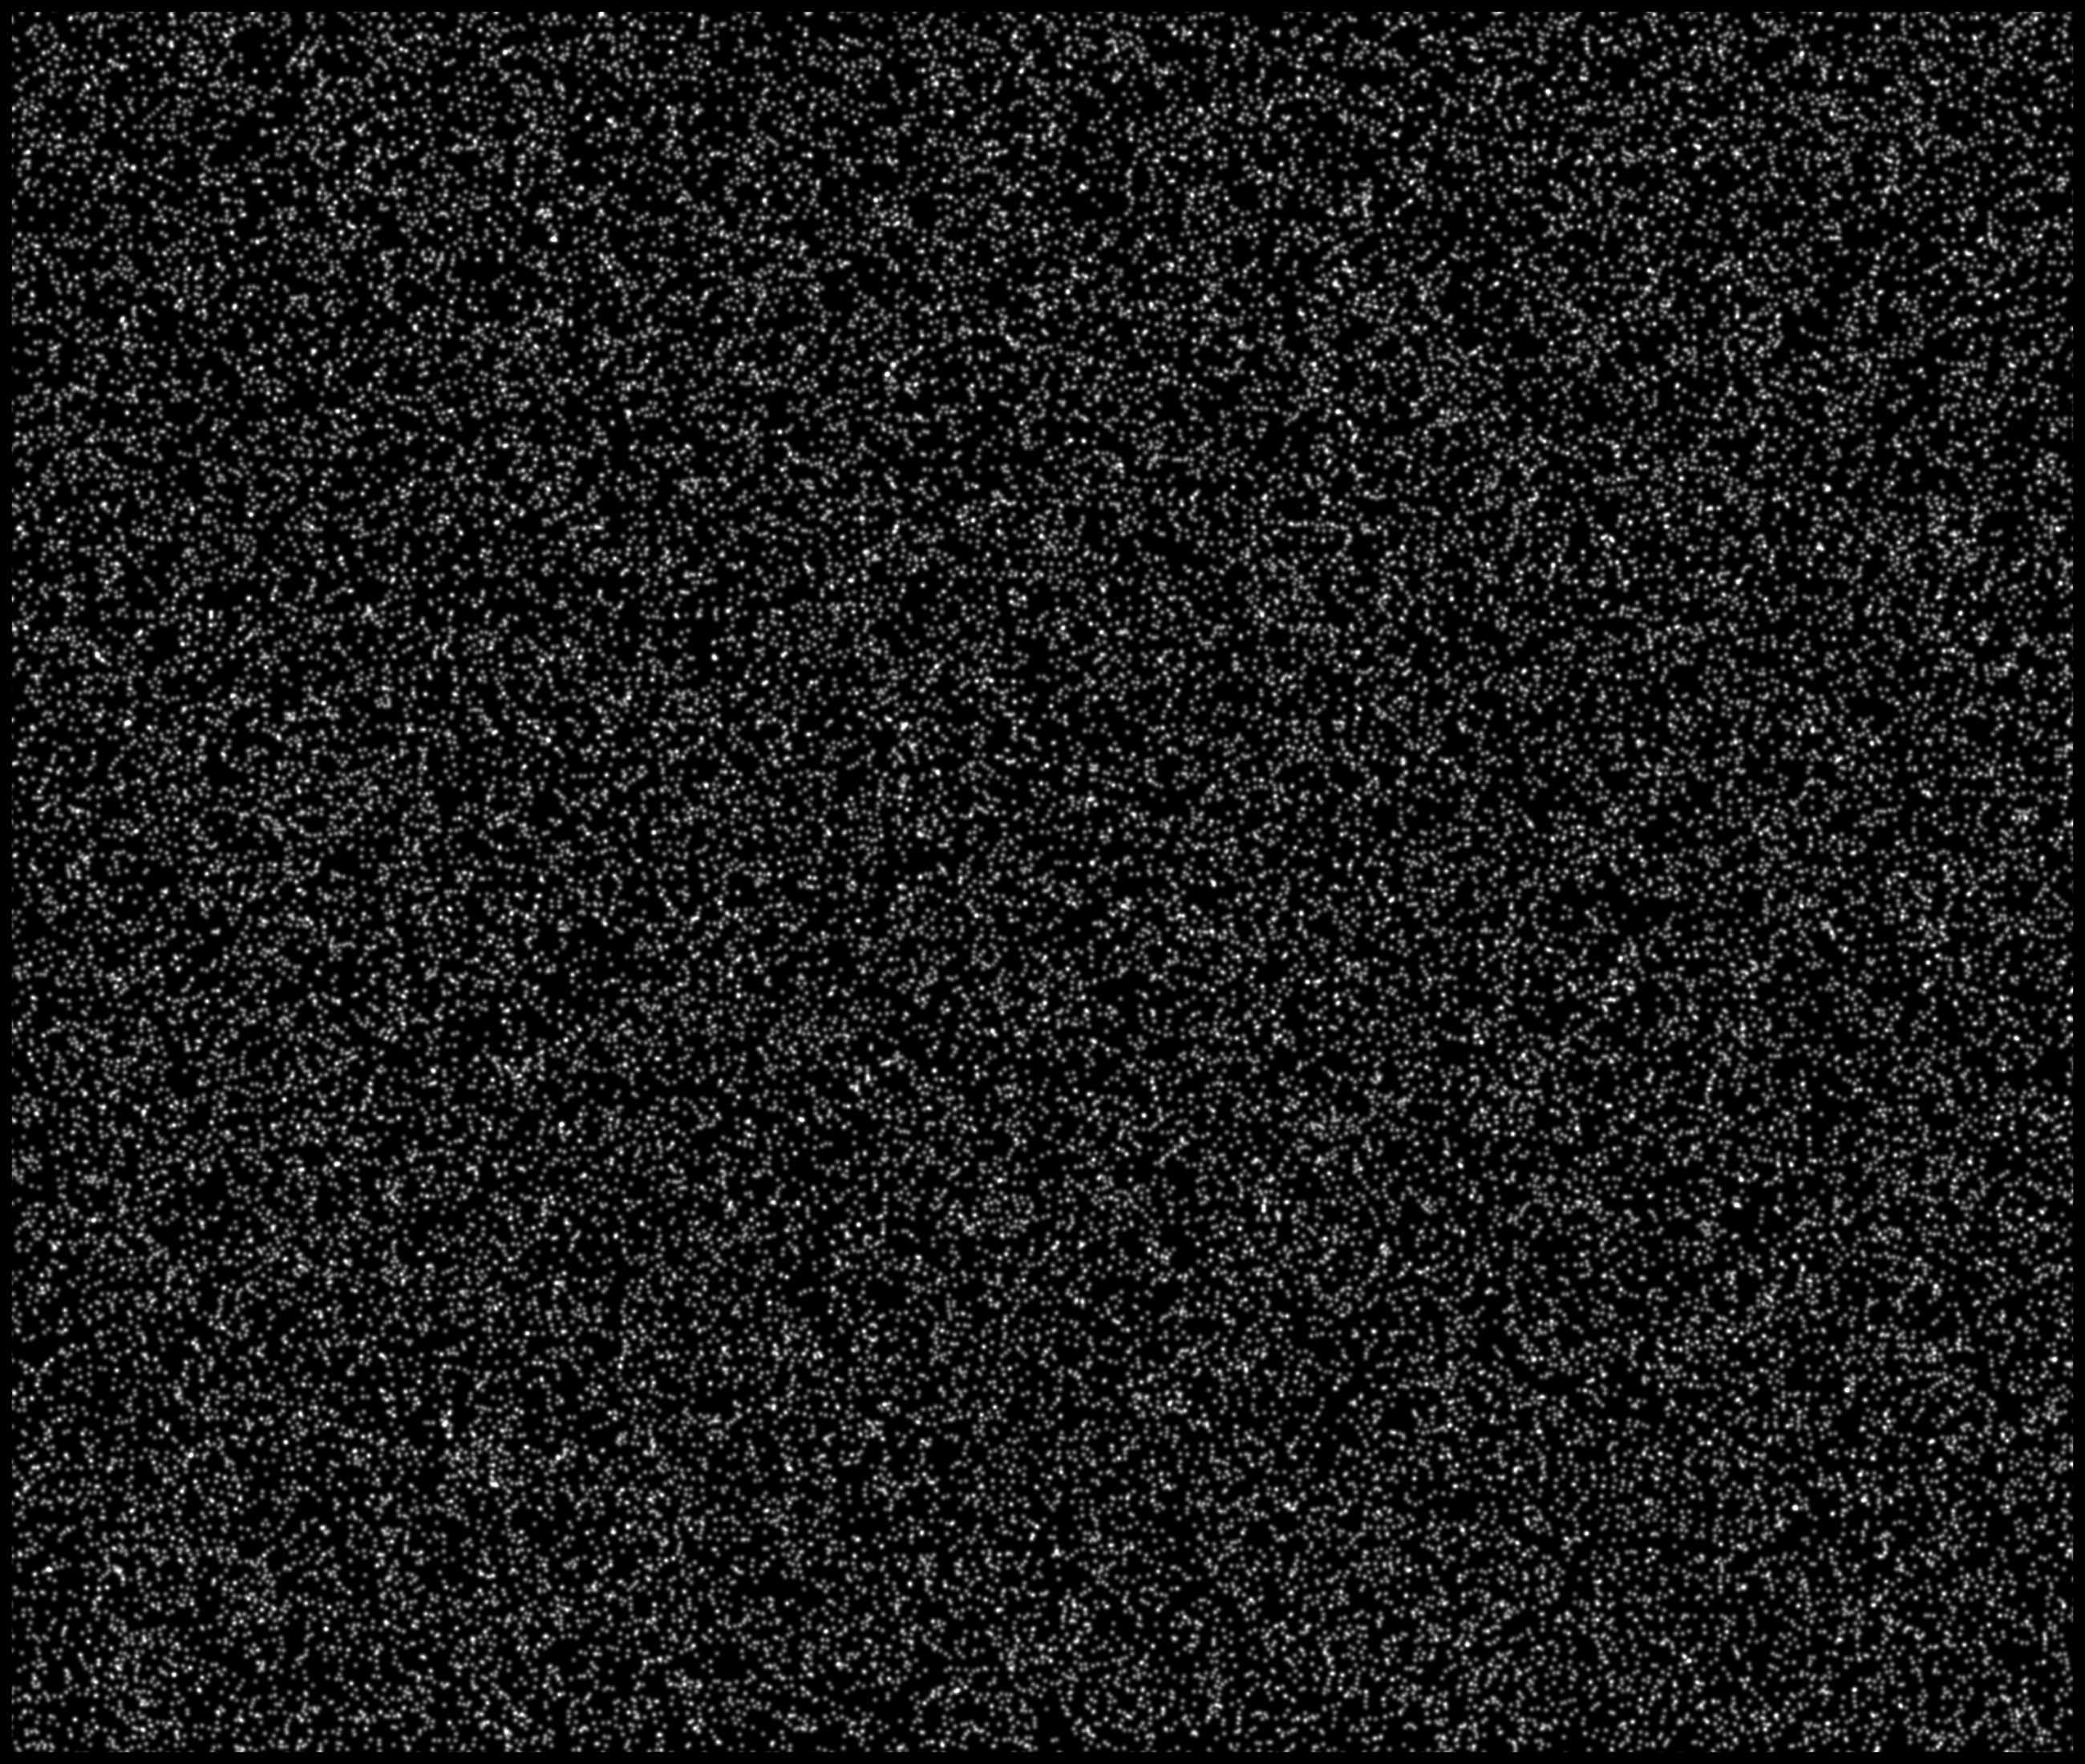
\includegraphics[scale=3.0]{./figures/04sypiv/0_1_150000.tif}
        \caption{Synthetic image - i}
        \label{fig:0_1_150000}
    \end{subfigure}%
    \begin{subfigure}{0.5\textwidth}
        \centering
        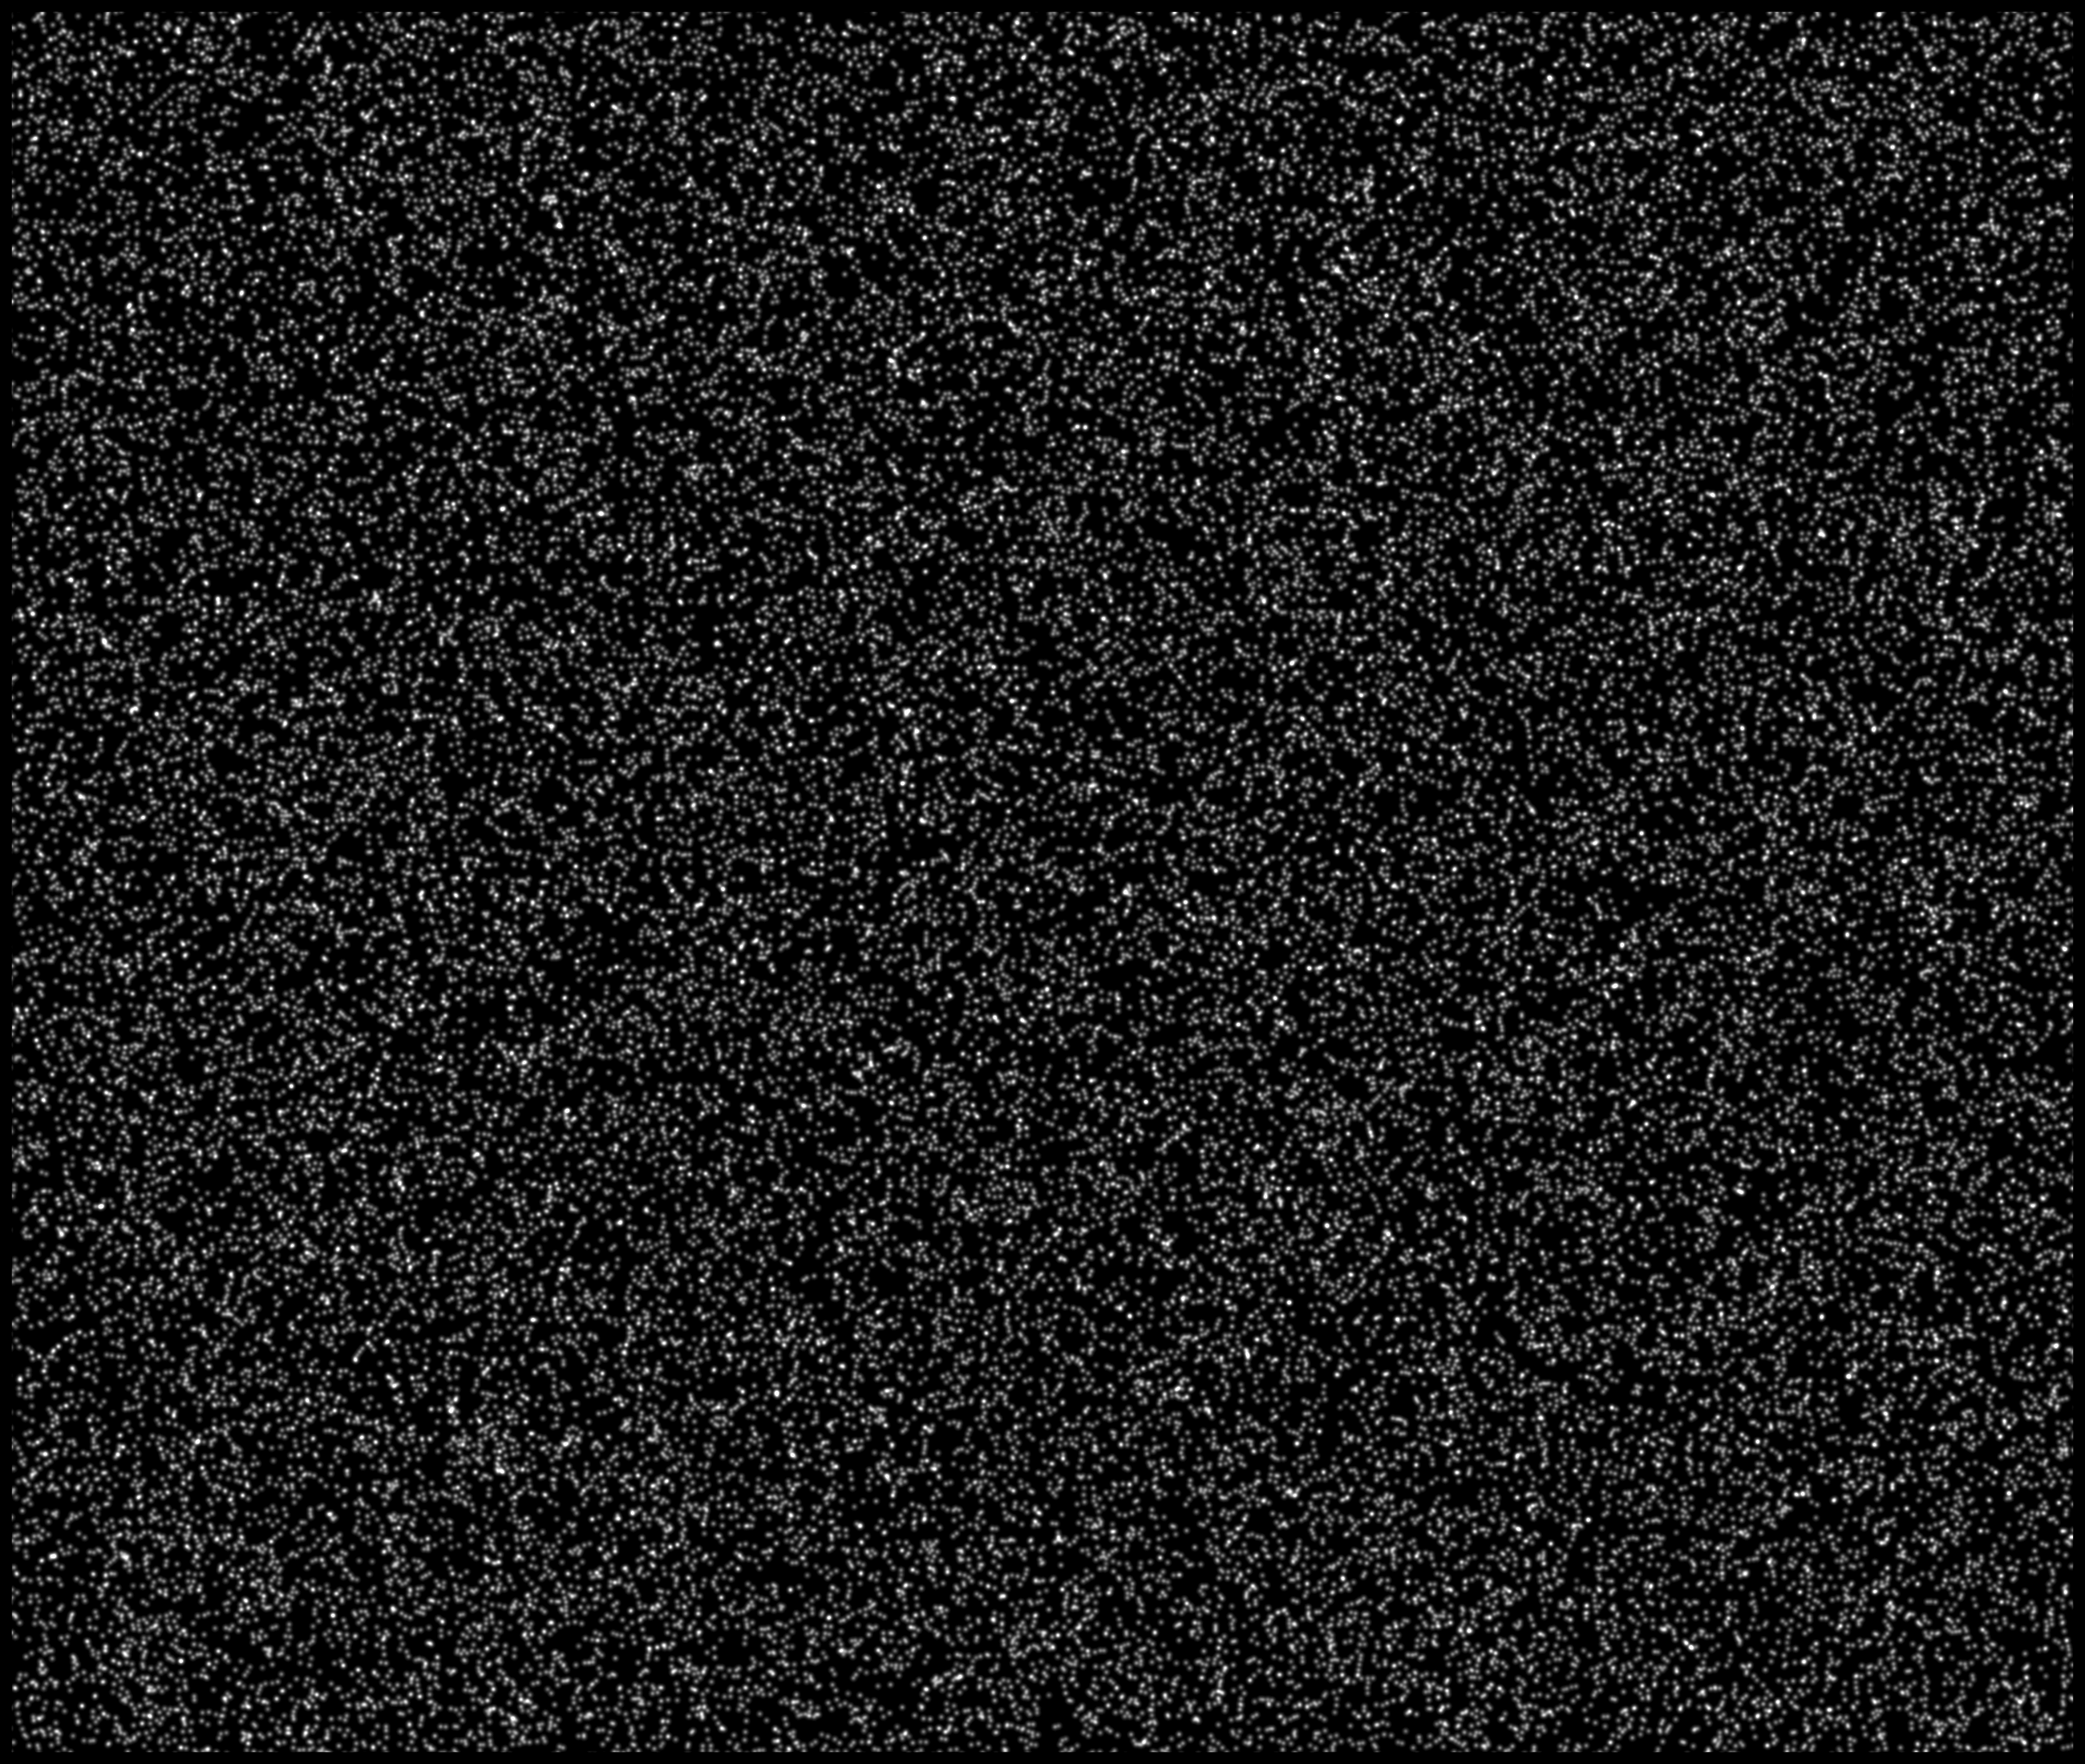
\includegraphics[scale=3.0]{./figures/04sypiv/0_2_150000.tif}
        \caption{Synthetic image - ii}
        \label{fig:0_2_150000}
    \end{subfigure}
    \caption{A pair of synthetic images generated from the current syPIV code}
    \label{fig:sypiv_williams}
\end{figure}

\begin{table}[ht!]
\centering
\begin{tabular}{|c|c|}
\hline
\textbf{Parameter}           & \textbf{Value}  \\ \hline
Particle concentration       & 0.026 per pixel \\ \hline
Total particles              & 150000          \\ \hline
Particle distribution        & Uniform         \\ \hline
Sensor resolution            & 2600 x 2200     \\ \hline
Interframe time              & 180 ns          \\ \hline
In-plane particles           & 70\%            \\ \hline
DPI of the image             & 105 pixels/mm   \\ \hline
Laser thickness              & 1 mm            \\ \hline
In-plane particles           & 70\%            \\ \hline
IA bounds - shock normal     & [-5, 21] mm     \\ \hline
IA bounds - shock tangential & [24.3, 26.5] mm \\ \hline
\end{tabular}
\caption{Parameters used to generate synthetic images from analytical and corresponding PDH-informed data}
\label{tab:sypiv_parameters}
\end{table}

Synthetic images were generated for two data sets. One set of images was obtained for the analytical data, and the other for the PDH-informed data obtained from the LPT code. The initial locations of the particles in both images were kept constant to generate the same first snapshot. The second snapshot of the synthetic images was generated independently by integrating with the data from the respective sets. When overlaid, these images highlight the particle lag across the oblique shock in the dataset. The color-temperature-corrected overlapped images are presented in Fig. \ref{fig:overlapped_zoom} that highlights this particle lag as streaks. The streaks are clearer at the shock interface, highlighting the effect of particle inertia in the PDH-informed data. The particles around this region have moved farther after crossing the shock compared to the respective particles in the image obtained from the analytical data, causing the streak effect observed in the zoomed portion of the image.\par

\begin{figure}[ht!]
    \centering
    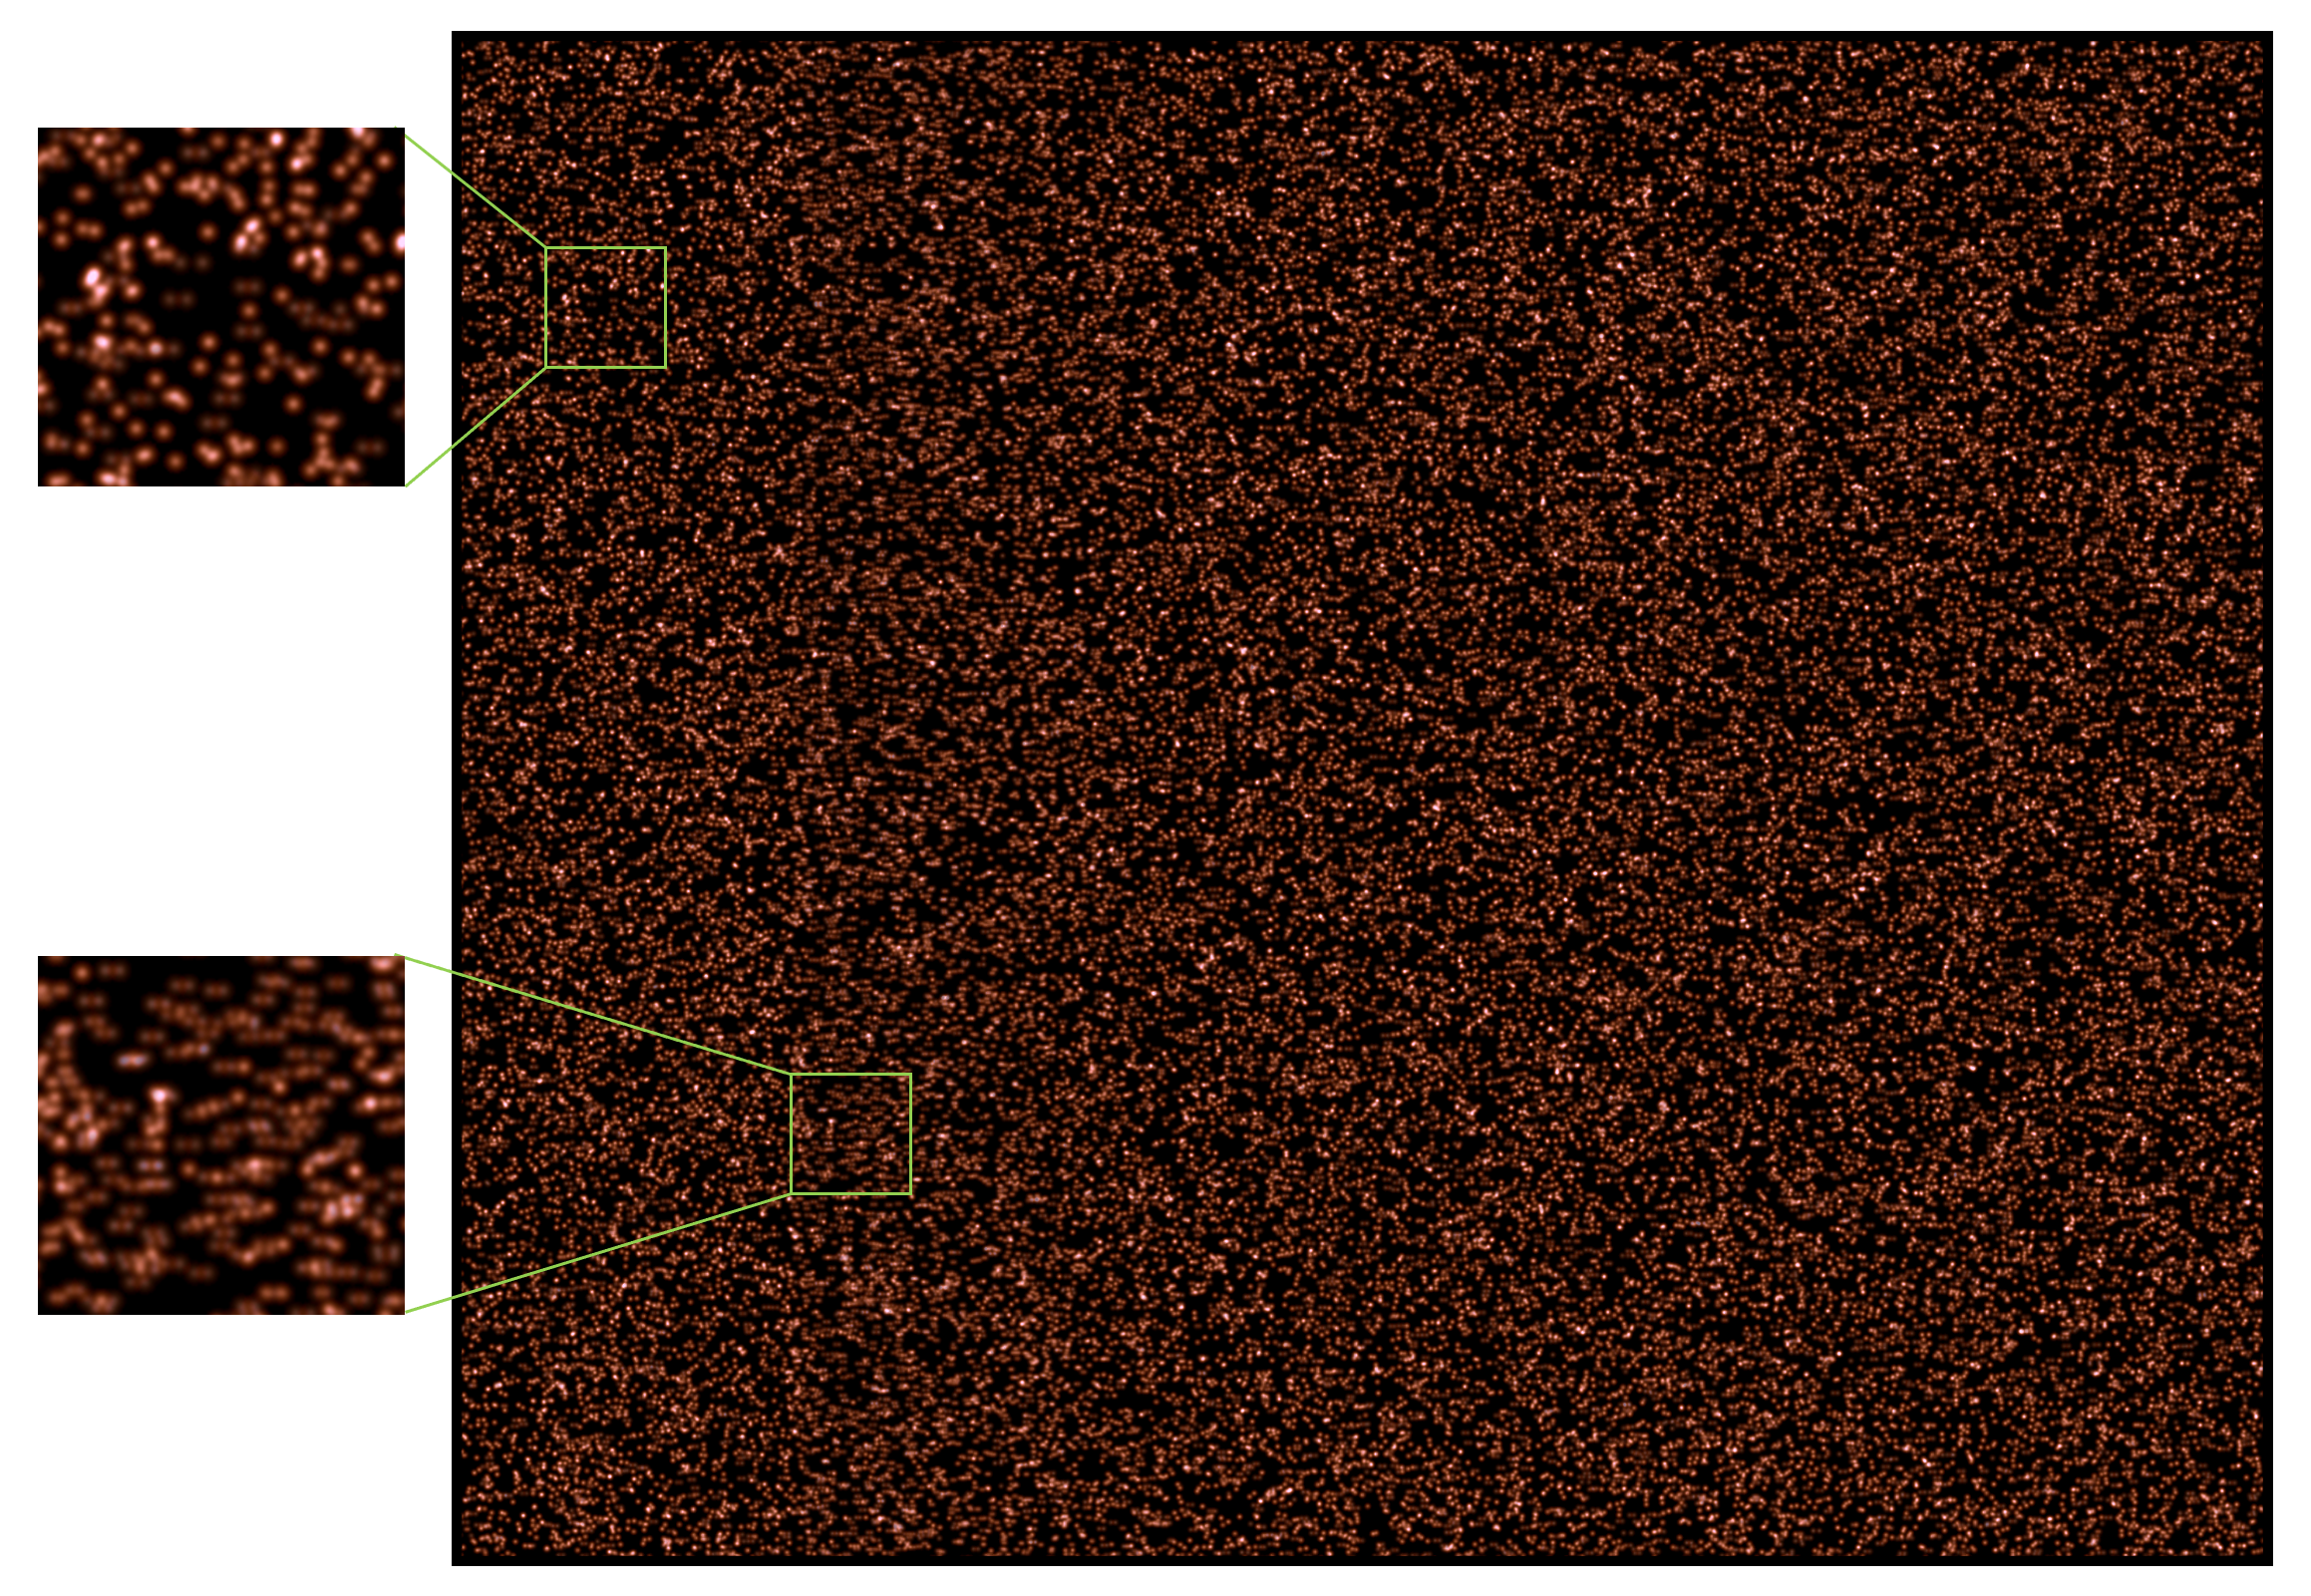
\includegraphics[scale=0.4]{./figures/04sypiv/overlapped_zoom.tiff}
    \caption{Overlapped second snapshots of synthetic images generated from the analytical data and respective PDH informed data highlighting the effect of PDH that shows up as streaks}
    \label{fig:overlapped_zoom}
\end{figure}

The images obtained from the syPIV code can be processed using any PIV data processing code. In this work, an open source code, open-PIV \cite{liberzon2020} is used because of its ease of implementation. The data was processed using a single-pass cross-correlation run. The default parameters are used for the signal-to-noise ratio and the correlation method for demonstration purposes. The velocity data were obtained using an interrogation window size of 48x48, which agrees with the PIV analysis of Williams et al. \cite{williams2015}. The processed vector field for both the analytical and PDH-informed data is overlayed in Fig. \ref{fig:vector_overlap}. This highlights the effect of particle presence on optical velocimetry data, providing a qualitative understanding of the impact of particle presence.\par

\begin{figure}[ht!]
    \centering
    \includesvg[scale=0.7]{./figures/04sypiv/quiver_comparison}
    \caption{Overlapped velocity vectors obtained by processing synthetic images}
    \label{fig:vector_overlap}
\end{figure}

For the current analysis, no image averaging was performed. Instead, better statistics were obtained by converting the data to a one-dimensional format by averaging along Y locations. Comparison of the shock normal velocity lag data is presented in Fig. \ref{fig:velocity_comparison}. The contrast between PDH-informed data and traditional data makes the importance of PDH evident when analyzing flow fields using synthetic images, as in the case of numerical code validation. This is especially true in supersonic flows, as shown here.\par

\begin{figure}[ht!]
    \centering
    \begin{subfigure}{0.5\textwidth}
        \centering
        \includesvg[width=0.9\linewidth]{./figures/04sypiv/syPIV_validation}
        \caption{Shock normal velocity lag}
        \label{fig:velocity_comparison}
    \end{subfigure}%
    \begin{subfigure}{0.5\textwidth}
        \centering
        \includesvg[width=0.9\linewidth]{./figures/04sypiv/validation_error}
        \caption{Error in velocity}
        \label{fig:velocity_error}
    \end{subfigure}
    \caption{Validation of numerical and syPIV models to experimental data}
    \label{fig:validation}
\end{figure}

The error in the shock normal velocity lag between the LPT code, the PDH-informed syPIV, and the traditional way of generating syPIV is presented in Fig. \ref{fig:velocity_error}. The average error computed as the RMS between the data sets from 0 to 20mm is detailed below:

\begin{enumerate}
    \item between the traditional syPIV and experiment is 15.8\%
    \item between the numerical particle track (LPT code) and experiment is 0.6\%
    \item between the PDH-informed data and experiment is 0.2\%
\end{enumerate}

\noindent The maximum error computed as the relative difference between the data sets is:

\begin{enumerate}
    \item between the traditional syPIV and experiment is 86\%
    \item between the LPT code and experiment is 2\%
    \item between the PDH-informed data and experiment is 1.7\%
\end{enumerate}

Traditional syPIV data have the inherent assumption that the particles carry the local flow velocity in the first image, leading to a huge average error in the velocity lag compared to the LPT code and PDH-informed data. The difference in error between the PDH-informed data and the numerical code suggests that the image analysis did not produce any significant uncertainty in this current case. When studying flows with tracers, the maximum error values show that PDH is locally substantial in acceleration regions.\par

\section{Summary}
A module for generating synthetic planar PIV images has been explored. Each aspect of PIV, such as the tracer particles, interrogation area, laser sheet, and optics, has been carefully modeled. Several test cases were used to verify the current code. These test cases explored the parameters of the code responsible for particle diameter and intensity. This helped to understand the default parameters to be used for synthetic image generation in real-world cases.

Synthetic Image Generation (SIG) for PIV has traditionally been used to verify PIV algorithms and validate numerical codes because it captures particle lag. The traditional approach, however, does not capture the particle dynamics history (PDH). The PDH has been explained in Chapter \ref{ch:pdh}. The entire process for generating PDH-informed PIV images has been validated against the shock response analysis of Williams et al. \cite{williams2015}. The qualitative data reported highlighted PDH in the oblique shock region. The average and maximum errors obtained showed the importance of reporting errors locally to understand the impact of PDH on the data obtained from PIV.
